% \iffalse meta-comment
%
% Copyright (C) 2015-2020 by Josef Friedrich <josef@friedrich.rocks>
% ----------------------------------------------------------------------
% This work may be distributed and/or modified under the conditions of
% the LaTeX Project Public License, either version 1.3 of this license
% or (at your option) any later version.  The latest version of this
% license is in:
%
%   http://www.latex-project.org/lppl.txt
%
% and version 1.3 or later is part of all distributions of LaTeX
% version 2005/12/01 or later.
%
% This work has the LPPL maintenance status `maintained'.
%
% The Current Maintainer of this work is Josef Friedrich.
%
% This work consists of the files cloze.dtx and cloze.ins
% and the derived filebase cloze.sty and cloze.lua.
%
% \fi
%
% \iffalse
%<*driver>
\ProvidesFile{cloze.dtx}
%</driver>
%<package>\NeedsTeXFormat{LaTeX2e}[1999/12/01]
%<package>\ProvidesPackage{cloze}
%<*package>
    [2020/05/27 v1.5 Package to typeset cloze worksheets or cloze tests]
%</package>
%<*driver>
\documentclass{ltxdoc}
\usepackage[show]{cloze}
\usepackage{graphicx}
\usepackage{paralist}
\usepackage{titlesec}
\usepackage{mdframed}
\titleformat{\paragraph}[hang]{%
  \normalfont\normalsize\bfseries%
  }{\theparagraph}{1em}{}
\titleformat{\subparagraph}[hang]{%
  \normalfont\small\bfseries%
  }{\thesubparagraph}{1em}{}
  \titlespacing*{\subparagraph}{0pt}{*1}{0pt}

\usepackage[
  colorlinks=true,
  linkcolor=red,
  filecolor=red,
  urlcolor=red,
]{hyperref}

\usepackage{minted}
\usemintedstyle{colorful}
\BeforeBeginEnvironment{minted}{\begin{mdframed}[backgroundcolor=gray!3]}
\AfterEndEnvironment{minted}{\end{mdframed}}
\setminted{
  breaklines=true,
  fontsize=\footnotesize,
}


\MakeShortVerb{\|}

\setlength{\fboxrule}{0.2pt}
\setlength{\fboxsep}{4pt}

\makeatletter
\newcommand{\@minipagerestore}{\setlength{\parindent}{10pt}}
\makeatother

\newmdenv{example}
\definecolor{graybackground}{gray}{0.97}
\surroundwithmdframed[backgroundcolor=graybackground]{verbatim}

\newcommand{\getdefaults}[1]{%
  \directlua{tex.print(cloze.get_defaults('#1'))}%
}

\newcommand{\expdesc}[1]{(|#1|)}

\newcommand{\desc}[1]{%
  \hfill%
  \expdesc{#1}%
  \par%
}

\def\tt#1{\texttt{#1}}

\def\secref#1{(\rightarrow\ \ref{#1})}

\newcommand{\option}[2]{\tt{[#1=}\meta{#2}\tt{]}}
\newcommand{\clozeluafunction}[1]{
  \marginpar{%
    \raggedleft%
    \MacroFont%
    \tt{%
      \scantokens{\catcode`\_=12\relax#1}%
    }%
  }%
}

\newcommand{\nodelisthfont}{\bfseries\sffamily}

\newcommand{\nodelistheader}{
  \hline
  \nodelisthfont Variable name &
  \nodelisthfont Node type &
  \nodelisthfont Node subtype &
  \nodelisthfont Parameter \\
  \hline
}

\newenvironment{nodelist}{
  \noindent
  \begingroup
  \footnotesize
  \begin{tabular}{llll}
  \nodelistheader
}{
  \hline
  \end{tabular}
  \endgroup
}

\EnableCrossrefs
\CodelineIndex
\RecordChanges
\begin{document}

\providecommand*{\url}{\texttt}
\GetFileInfo{cloze.dtx}
\title{The \cloze{cloze} package%
  \thanks{Many thanks to Robert-Michael Huber for his advice
and to Paul Isambert for his article \emph{"Three things you can do with
Lua\TeX{} that would be extremely painful otherwise"} in TUGboat, Volume
31 (2010), No. 3. This article helped a lot to write this package.}%
}
\author{%
  Josef Friedrich\\%
  \url{josef@friedrich.rocks}\\%
  \href{https://github.com/Josef-Friedrich/cloze}{github.com/Josef-Friedrich/cloze}%
}
\date{\fileversion~from \filedate}

\maketitle\vfill

\pagebreak

\setcounter{secnumdepth}{5}
\setcounter{tocdepth}{5}
\tableofcontents

%-----------------------------------------------------------------------
% Introduction
%-----------------------------------------------------------------------

\pagebreak
\section{Introduction}

\emph{cloze} is a \LaTeX{} package to generate cloze texts. It uses
the capabilities of the modern \TeX{} engine \emph{Lua\TeX}. Therefore,
you must use Lua\LaTeX{} to create documents containing gaps.

\begin{verbatim}
lualatex cloze-text.tex
\end{verbatim}

The main feature of the package is that the formatting doesn't change
when using the |hide| and |show| \secref{sec:option-hide} options.

\newcommand{\clozelorem}{%
Lorem ipsum \cloze{dolor sit} amet, consectetur \cloze{adipisicing}
elit, sed do eiusmod tempor incididunt ut labore et \cloze{dolore magna}
aliqua. Ut enim ad minim veniam, quis nostrud \cloze{exercitation}
ullamco laboris nisi ut \cloze{aliquip} ex ea commodo consequat.%
}

\begin{example}
\clozelorem
\end{example}

\clozeset{hide}

The command |\clozeset{hide}| only shows gaps. When you put both texts
on top of each other you will see that they perfectly match.

\begin{example}
\clozelorem
\end{example}

\clozeset{show}

%-----------------------------------------------------------------------
% Usage
%-----------------------------------------------------------------------

\section{Usage}

There are the commands
\cmd{\cloze},
\cmd{\clozefix},
\cmd{\clozefil},
\cmd{\clozenol},
\cmd{\clozestrike} and the environments
|clozepar| and
|clozebox|
to generate cloze texts.

%%
% \cloze
%%

\subsection{The commands and environments}

\subsubsection{\cmd{\cloze}}
\label{sec:command-cloze}

\DescribeMacro{\cloze} \cmd{\cloze}\oarg{options}\marg{some text}: The
command \cmd{\cloze} is similar to a command that offers the possibility
to underline the texts. \cmd{\cloze} does not prevent line breaks. The
width of a gap depends on the number of letters and the font used.
The only option which affects the widths of a gap is the option
|margin| \secref{sec:option-margin}.

\begin{example}
Lorem ipsum \cloze{dolor} sit amet, \cloze{consectetur} adipisicing
elit, sed do eiusmod tempor incididunt ut labore et dolore
\cloze{magna aliqua. Ut enim ad minim veniam, quis nostrud exercitation
ullamco laboris nisi} ut aliquip ex ea commodo consequat.
\end{example}

\noindent It is possible to convert a complete paragraph into a `gap'.
But don't forget: There is a special environment for this: \tt{clozepar}
\secref{sec:command-clozepar}.

\begin{example}
\cloze{Lorem ipsum dolor sit amet, consectetur adipisicing elit, sed do
eiusmod tempor incididunt ut labore et dolore magna aliqua. Ut enim ad
minim veniam, quis nostrud exercitation ullamco laboris nisi ut aliquip
ex ea commodo consequat.}
\end{example}

\noindent The command \cmd{\cloze} doesn't change the behavior of the
hyphenation. Let's try some long German words:

\begin{example}
es
\cloze{Te\-le\-kom\-mu\-ni\-ka\-tions\-ü\-ber\-wach\-ung}
geht
\cloze{Un\-ter\-neh\-mens\-steu\-er\-fort\-ent\-wick\-lungs\-ge\-setz}
\cloze{Ab\-teil\-ungs\-lei\-ter\-in}
\cloze{Ober\-kom\-mi\-sar\-in}
auch
\cloze{Fil\-lial\-lei\-ter\-in}
kurz
\cloze{Ober\-kom\-mi\-sar\-in}
\cloze{Un\-ter\-neh\-mens\-steu\-er\-fort\-ent\-wick\-lungs\-ge\-setz}
\cloze{Fil\-lial\-lei\-ter\-in}
\cloze{Metz\-ger\-mei\-ster\-in}
in
\cloze{Ab\-teil\-ungs\-lei\-ter\-in}
der
\cloze{Ober\-kom\-mi\-sar\-in}
\cloze{Hoch\-lei\-stungs\-flüs\-sig\-keits\-chro\-ma\-to\-gra\-phie}
\cloze{Fil\-lial\-lei\-ter\-in}
Kürze
\cloze{Un\-ter\-neh\-mens\-steu\-er\-fort\-ent\-wick\-lungs\-ge\-setz}
\cloze{Metz\-ger\-mei\-ster\-in}
liegt
\cloze{Ab\-teil\-ungs\-lei\-ter\-in}
die
\cloze{Metz\-ger\-mei\-ster\-in}
\cloze{Ab\-teil\-ungs\-lei\-ter\-in}
Würze
\cloze{Ober\-kom\-mi\-sar\-in}
\end{example}

%%
% \clozesetfont
%%

\subsubsection{\cmd{\clozesetfont}}
\label{sec:command-clozesetfont}
\label{sec:command-clozefont}

\DescribeMacro{\clozesetfont}
The gap font can be changed by using the command
\cmd{\clozesetfont}. \tt{\string\cloze\-set\-font} redefines the command
\cmd{\clozefont} which contains the font definition.
Thus, the command \tt{\string\clozesetfont\string{\string\Large\string}}
has the same effect as
\tt{\string\re\-new\-com\-mand\string{\string\cloze\-font\string}%
\string{\string\Large\string}}.

\clozesetfont{\Large}

\begin{example}
Excepteur \cloze{sint} occaecat \cloze{cupidatat} non proident.
\end{example}

\noindent Please do not put any color definitions in
\cmd{\clozesetfont}, as it won't work. Use the option
|textcolor| instead \secref{sec:option-textcolor}.

|\clozesetfont{\ttfamily\normalsize}| changes the gap text for example
into a normal sized typewriter font.

\clozesetfont{\ttfamily\normalsize}

\begin{example}
Excepteur \cloze{sint} occaecat \cloze{cupidatat} non proident.
\end{example}

\clozesetfont{\itshape}

%%
% \clozefix
%%

\subsubsection{\cmd{\clozefix}}
\label{sec:command-clozefix}

\DescribeMacro{\clozefix} \cmd{\clozefix}\oarg{options}\marg{some text}:
The command \cmd{\clozefix} creates gaps with a fixed width. The
clozes are default concering the width \tt{\getdefaults{width}}.

\begin{example}
\noindent Lorem ipsum dolor sit amet:
\begin{compactenum}
\item \clozefix[width=5cm]{consectetur}
\item \clozefix[width=5cm]{adipisicing}
\item \clozefix[width=5cm]{elit}
\end{compactenum}
sed do eiusmod.
\end{example}

Gaps with a fixed width are much harder to solve.

\begin{example}
Lorem ipsum dolor \clozefix[align=center,width=3cm]{sit} amet,
\clozefix[align=center,width=3cm]{consectetur} adipisicing elit, sed do
eiusmod tempor incididunt \clozefix[align=center,width=3cm]{ut} labore
et dolore magna aliqua.
\end{example}

Using the option |align| you can make nice tabulars like this:

\begin{example}
\begin{tabular}{p{5cm}p{4cm}}
\raggedleft Composer & Life span \\
\clozefix[width=5cm,align=right]{Joseph Haydn} & \clozefix{1723-1809} \\
\clozefix[width=5cm,align=right]{Wolfgang Amadeus Mozart} & \clozefix{1756-1791} \\
\clozefix[width=5cm,align=right]{Ludwig van Beethoven} & \clozefix{1770-1827} \\
\end{tabular}
\end{example}

%%
% \clozenol
%%

\subsubsection{\cmd{\clozenol}}
\label{sec:command-clozenol}
\DescribeMacro{\clozenol} \cmd{\clozenol}\oarg{options}\marg{some text}:
The macro name |clozenol| stands for \emph{“cloze no line”}. As the
the name suggests this macro typesets cloze texts without a line.

\begin{minted}{latex}
Lorem \clozenol{ipsum dolor} sit amet.
\end{minted}

\begin{example}
Lorem \clozenol{ipsum dolor} sit amet.
\end{example}

\begin{minted}{latex}
Lorem \clozenol[textcolor=green]{ipsum dolor} sit amet.
\end{minted}

\begin{example}
Lorem \clozenol[textcolor=green]{ipsum dolor} sit amet.
\end{example}

%%
% \clozefil
%%

\subsubsection{\cmd{\clozefil}}
\label{sec:command-clozefil}

\DescribeMacro{\clozefil} \cmd{\clozefil}\oarg{options}\marg{some text}:
The name of the command is inspired by \cmd{\hfil}, \cmd{\hfill}, and
\cmd{\hfilll}. Only \cmd{\clozefil} fills out all available horizontal
spaces with a line.

\begin{example}
Lorem ipsum dolor sit amet, \clozefil{consectetur adipisicing elit, sed
do eiusmod.}

Ut enim \clozefil{ad minim veniam} exercitation.
\end{example}

%%
% \clozeextend
%%

\subsubsection{\cmd{\clozeextend}}
\label{sec:command-clozeextend}

\DescribeMacro{\clozeextend} \cmd{\clozeextend}\oarg{spaces}:
The command |\clozeextend| adds some invisible placeholders to extend
some cloze texts with blank space.

\begin{minted}{latex}
\begin{itemize}
\item \clozefil{Lorem ipsum dolor sit amet, consectetur adipisicing
elit, sed do eiusmod tempor incididunt ut labore et dolore magna
aliqua.}
\item \clozefil{Ut enim ad minim veniam \clozeextend[20]}
\item \clozefil{quis nostrud \clozeextend[20]}
\end{itemize}
\end{minted}

\begin{example}
\begin{itemize}
\item \clozefil{Lorem ipsum dolor sit amet, consectetur adipisicing
elit, sed do eiusmod tempor incididunt ut labore et dolore magna
aliqua.}
\item \clozefil{Ut enim ad minim veniam \clozeextend[20]}
\item \clozefil{quis nostrud \clozeextend[20]}
\end{itemize}
\end{example}

%%
% clozepar
%%

\subsubsection{\tt{clozepar}}
\label{sec:command-clozepar}

\DescribeEnv{clozepar} |\begin{clozepar}|\oarg{options} \dots
\textit{some text} \dots |\end{clozepar}|: The environment \tt{clozepar}
transforms a complete paragraph into a cloze text. The options |align|,
|margin| and |width| have no effect on this environment.

\begin{example}
Lorem ipsum dolor sit amet, consectetur adipisicing elit ullamco laboris
nisi.

\begin{clozepar}
Ut enim ad minim veniam, quis nostrud exercitation ullamco laboris nisi
ut aliquip ex ea commodo consequat. Duis aute irure dolor in
reprehenderit in voluptate velit esse cillum.
\end{clozepar}

Excepteur sint occaecat cupidatat non proident.
\end{example}

%%
% clozebox
%%

\subsubsection{\tt{clozebox}}
\label{sec:command-clozebox}

\DescribeEnv{clozebox} |\begin{clozebox}|*\oarg{options} \dots
\textit{some text} \dots |\end{clozebox}|: The environment \tt{clozebox}
surrounds a text with a box. The starred version omits the line
around the box. Use the options |boxwidth| and |boxheight| to specify
the dimensions of the box. By default the width of the box is
|\linewidth|.

\begin{minted}{latex}
\begin{clozebox}
Lorem ipsum dolor sit amet, consectetur adipisicing elit, sed do eiusmod
tempor incididunt ut labore et dolore magna aliqua.
\end{clozebox}
\end{minted}

\bigskip
\noindent
|\clozehide|
\clozehide
\bigskip

\begin{center}
\begin{clozebox}[boxwidth=8cm]
Lorem ipsum dolor sit amet, consectetur adipisicing elit, sed do eiusmod
tempor incididunt ut labore et dolore magna aliqua.
\end{clozebox}
\end{center}

\bigskip
\noindent
|\clozeshow|
\clozeshow
\bigskip

\begin{center}
\begin{clozebox}[boxwidth=8cm]
Lorem ipsum dolor sit amet, consectetur adipisicing elit, sed do eiusmod
tempor incididunt ut labore et dolore magna aliqua.
\end{clozebox}
\end{center}

\paragraph{Option boxwidth}
\label{sec:command-clozebox-boxwidth}
See the documentation about the option \secref{sec:option-boxwidth}.

\begin{minted}{latex}
\begin{clozebox}[boxwidth=5cm]
Lorem ipsum dolor sit amet, consectetur adipisicing elit, sed do eiusmod
tempor incididunt ut labore et dolore magna aliqua.
\end{clozebox}
\end{minted}

\begin{center}
\begin{clozebox}[boxwidth=5cm]
Lorem ipsum dolor sit amet, consectetur adipisicing elit, sed do eiusmod
tempor incididunt ut labore et dolore magna aliqua.
\end{clozebox}
\end{center}

\paragraph{Option boxheight}
\label{sec:command-clozebox-boxheight}
See the documentation about the option \secref{sec:option-boxheight}.

\begin{minted}{latex}
\begin{clozebox}[boxwidth=5cm,boxheight=5cm]
Lorem ipsum dolor sit amet, consectetur adipisicing elit, sed do eiusmod
tempor incididunt ut labore et dolore magna aliqua.
\end{clozebox}
\end{minted}

\begin{center}
\begin{clozebox}[boxwidth=5cm,boxheight=5cm]
Lorem ipsum dolor sit amet, consectetur adipisicing elit, sed do eiusmod
tempor incididunt ut labore et dolore magna aliqua.
\end{clozebox}
\end{center}

\paragraph{starred}

% starred
\begin{minted}{latex}
\begin{clozebox}*[boxwidth=5cm,boxheight=5cm]
Lorem ipsum dolor sit amet, consectetur adipisicing elit, sed do eiusmod
tempor incididunt ut labore et dolore magna aliqua.
\end{clozebox}
\end{minted}

\begin{center}
\begin{clozebox}*[boxwidth=5cm,boxheight=5cm]
Lorem ipsum dolor sit amet, consectetur adipisicing elit, sed do eiusmod
tempor incididunt ut labore et dolore magna aliqua.
\end{clozebox}
\end{center}

%%
% clozespace
%%

\subsubsection{\tt{clozespace}}
\label{sec:command-clozespace}

\DescribeEnv{clozespace} |\begin{clozespace}|\oarg{options} \dots
\textit{some text} \dots |\end{clozespace}|

\begin{minted}{latex}
\begin{clozespace}[spacing=2]
\clozesetfont{\ttfamily\Huge}
Lorem \cloze{ipsum} dolor sit \cloze{amet}, consectetur adipisicing
elit, sed do eiusmod tempor incididunt ut labore et dolore magna
aliqua. Ut enim ad minim veniam, quis \cloze{nostrud}
exercitation ullamco \cloze{laboris} nisi ut aliquip ex ea commodo
consequat.
\end{clozespace}
\end{minted}

\begin{example}
\begin{clozespace}[spacing=2]
\clozesetfont{\ttfamily\Huge}
Lorem \cloze{ipsum} dolor sit \cloze{amet}, consectetur adipisicing
elit, sed do eiusmod tempor incididunt ut labore et dolore magna
aliqua. Ut enim ad minim veniam, quis \cloze{nostrud}
exercitation ullamco \cloze{laboris} nisi ut aliquip ex ea commodo
consequat.
\vspace{-0.8cm}
\end{clozespace}
\end{example}

%%
% \clozeline
%%

\subsubsection{\cmd{\clozeline}}
\label{sec:command-clozeline}

\DescribeMacro{\clozeline}
\cmd{\clozeline}\oarg{options}:
To create a cloze line of a certain width, use the command
\cmd{\clozeline}. The default width of the line is
\tt{\getdefaults{width}}. In combination with the other cloze commands
you can create for example an irregular alignment of the cloze text.

\begin{minted}{latex}
Ut enim ad
\clozeline[width=1cm]\cloze{minim}\clozeline[width=3cm]
minim veniam
\end{minted}

\begin{example}
Ut enim ad \clozeline[width=1cm]\cloze{minim}\clozeline[width=3cm] minim
veniam,
\end{example}

%%
% \clozelinefil
%%

\subsubsection{\cmd{\clozelinefil}}
\label{sec:command-clozelinefil}

\DescribeMacro{\clozelinefil}
\cmd{\clozelinefil}\oarg{options}:
This command \cmd{\clozelinefil} fills the
complete available horizontal space with a line. Moreover,
\cmd{\clozelinefil} was used to create \cmd{\clozefil}.

\begin{example}
Lorem\clozelinefil
\end{example}

%%
% \clozestrike
%%

\subsubsection{\cmd{\clozestrike}}
\label{sec:command-clozelinefil}

\DescribeMacro{\clozestrike}
\cmd{\clozestrike}\oarg{options}\marg{wrong text}\marg{correct text}

\begin{minted}{latex}
Lorem \clozestrike{ipsum}{dolor} sit amet.
\end{minted}

\begin{example}
Lorem \clozestrike{ipsum}{dolor} sit amet.
\end{example}

\begin{minted}{latex}
Lorem \clozestrike[textcolor=red]{ipsum}{dolor} sit amet.
\end{minted}

\begin{example}
Lorem \clozestrike[textcolor=red]{ipsum}{dolor} sit amet.
\end{example}

\begin{example}
\begin{clozespace}
invidunt ut \clozestrike{labore}{et dolore magna aliquyam erat}, sed
diam voluptua. At \clozestrike{vero eos}{et accusam et justo} duo
dolores et ea \clozestrike{rebum. Stet}{clita kasd gubergren}, no sea
takimata sanctus est Lorem ipsum dolor sit amet. Lorem ipsum
\clozestrike{dolor sit amet, consetetur }{sadipscing elitr, sed diam}
nonumy eirmod tempor invidunt ut labore et dolore magna
aliquyam erat, \clozestrike{sed diam voluptua}{At vero}.
\end{clozespace}
\end{example}

\begin{example}
\clozehide
\begin{clozespace}
invidunt ut \clozestrike{labore}{et dolore magna aliquyam erat}, sed
diam voluptua. At \clozestrike{vero eos}{et accusam et justo} duo
dolores et ea \clozestrike{rebum. Stet}{clita kasd gubergren}, no sea
takimata sanctus est Lorem ipsum dolor sit amet. Lorem ipsum
\clozestrike{dolor sit amet, consetetur }{sadipscing elitr, sed diam}
nonumy eirmod tempor invidunt ut labore et dolore magna
aliquyam erat, \clozestrike{sed diam voluptua}{At vero}.
\end{clozespace}
\clozeshow
\end{example}

%-----------------------------------------------------------------------
% Options
%-----------------------------------------------------------------------

\subsection{The options}

%%
% Local and global options
%%

\subsubsection{Local and global options}

The \emph{cloze} package distinguishs between \emph{local} and
\emph{global} options. Besides the possiblity to set \emph{global}
options in the \cmd{\usepackage}\oarg{global options}\marg{cloze}
declaration, the cloze package offers a special command to set
\emph{global} options:
\cmd{\clozeset}\marg{global options}

%%
% \clozeset
%%

\subsubsection{\cmd{\clozeset}}
\label{sec:command-clozeset}

\DescribeMacro{\clozeset}
\cmd{\clozeset}\marg{global options}: The command can set \emph{global}
options for each paragraph.

\begin{minted}{latex}
\clozeset{textcolor=red} Lorem \cloze{ipsum} dolor \par
\clozeset{textcolor=green} Lorem \cloze{ipsum} dolor
\end{minted}

\begin{example}
\clozeset{textcolor=red} Lorem \cloze{ipsum} dolor \par
\clozeset{textcolor=green} Lorem \cloze{ipsum} dolor
\end{example}

\noindent \cmd{\clozeset} does not change the options within a
paragraph. As you can see in the example below the last \cmd{\clozeset}
applies the color green for both gaps.

\begin{minted}{latex}
\clozeset{textcolor=red} Lorem \cloze{ipsum} dolor
\clozeset{textcolor=green} Lorem \cloze{ipsum} dolor
\end{minted}

\begin{example}
\clozeset{textcolor=red} Lorem \cloze{ipsum} dolor
\clozeset{textcolor=green} Lorem \cloze{ipsum} dolor
\end{example}

\clozereset

%%
% \clozereset
%%

\subsubsection{\cmd{\clozereset}}
\label{sec:command-clozereset}

\DescribeMacro{\clozereset}
\cmd{\clozereset}: The command resets all \emph{global} options to the
default values. It has no effect on the \emph{local} options.

\begin{minted}{latex}
\clozeset{
  thickness=3mm,
  linecolor=yellow,
  textcolor=magenta,
  margin=-2pt
}
\end{minted}

\clozeset{thickness=3mm,linecolor=yellow,textcolor=magenta,margin=-2pt}

\begin{example}
Very \cloze{silly} global \cloze{options}.
\end{example}

\begin{minted}{latex}
\clozereset
\end{minted}
\clozereset

\begin{example}
\cloze{Relax!} We can reset \cloze{those} options.
\end{example}

%%
% \clozereset
%%

\subsubsection{\cmd{\clozeshow} and \cmd{\clozehide}}
\label{sec:command-clozeshow}
\label{sec:command-clozehide}

\DescribeMacro{\clozeshow} \DescribeMacro{\clozehide}
\cmd{\clozeshow} and \cmd{\clozehide}: This commands are shortcuts for
\cmd{\clozeset}\marg{show} and \cmd{\clozeset}\marg{hide}.

\begin{minted}{latex}
\clozehide
\end{minted}
\clozehide

\begin{example}
Lorem \cloze{ipsum dolor sit} amet, consectetur \cloze{adipisicing}
elit.
\end{example}

\begin{minted}{latex}
\clozeshow
\end{minted}
\clozeshow

\begin{example}
Lorem \cloze{ipsum dolor sit} amet, consectetur \cloze{adipisicing}
elit.
\end{example}

%%
% align
%%

\subsubsection{\tt{align}}
\label{sec:option-align}

\option{align}{left/center/right}:
Only the macro \cmd{\clozefix} \secref{sec:command-clozefix} takes the
option \tt{align} into account. Possible values are \tt{left},
\tt{center} and \tt{right}. This option only makes sense, if the width
of the line is larger than the width of the text.

\newcommand{\optionsalign}[1]{%
  \noindent%
  \clozefix[align=#1,width=8cm]{Lorem ipsum}%
  \desc{#1}%
}

\begin{example}
\optionsalign{left}
\optionsalign{center}
\optionsalign{right}
\end{example}

%%
% boxheight
%%

\subsubsection{\tt{boxheight}}
\label{sec:option-boxheight}

|boxheight| specifies the height of a cloze box. This option has only
an effect on the environment |clozebox| \secref{sec:command-clozebox}.
An example can be found in the section about the environment
\secref{sec:command-clozebox-boxheight}.

%%
% boxwidth
%%

\subsubsection{\tt{boxwidth}}
\label{sec:option-boxwidth}

|boxwidth| specifies the width of a cloze box. This option has only
an effect on the environment |clozebox| \secref{sec:command-clozebox}.
An example can be found in the section about the environment
\secref{sec:command-clozebox-boxwidth}.

%%
% distance
%%

\subsubsection{\tt{distance}}
\label{sec:option-distance}

\option{distance}{dimen}:
The option |distance| specifies the spacing between the baseline of the
text and the gap line. The larger the dimension of the option
|distance|, the more moves the line down. Negative values cause the line
to appear above the baseline. The default value is
\tt{\getdefaults{distance}}.

\newcommand{\optiondistance}[1]{%
  \noindent%
  \clozefil[distance=#1]{Lorem ipsum dolor sit amet.}
  \expdesc{#1}
  \par%
}

\begin{example}
\optiondistance{\getdefaults{distance}}
\optiondistance{3pt}
\optiondistance{-3pt}
\end{example}

%%
% hide and show
%%

\subsubsection{\tt{hide} and \tt{show}}
\label{sec:option-hide}
\label{sec:option-show}

\tt{[hide]} and \tt{[show]}:
By default the cloze text is displayed. Use the option |hide| to remove
the cloze text from the output.  If you accidentally specify both
options -- |hide| and |show| -- the last option "wins".

\newcommand{\optionshow}[1]{%
  \noindent%
  Lorem ipsum \cloze[#1]{dolor sit amet}, consectetur
  \cloze[#1]{adipisicing} elit.%
  \desc{#1}%
}

\begin{example}
\optionshow{hide}
\optionshow{show}
\optionshow{show,hide}
\optionshow{hide,show}
\end{example}

%%
% linecolor and textcolor
%%

\subsubsection{\tt{linecolor} and \tt{textcolor}}
\label{sec:option-linecolor}
\label{sec:option-textcolor}

\option{linecolor}{color name} and
\option{textcolor}{color name}:
Values for both color options are color names used by the xcolor
package. To define your own color use the following command:

\begin{minted}{latex}
\definecolor{myclozecolor}{rgb}{0.1,0.4,0.6}
\cloze[textcolor=myclozecolor]{Lorem ipsum}
\end{minted}
\definecolor{myclozecolor}{rgb}{0.1,0.4,0.6}

\newcommand{\optioncolor}[2]{%
  \noindent%
  \clozefil[#1=#2]{Lorem ipsum dolor sit amet, consectetur} %
  \expdesc{#2}%
  \par%
}

\begin{example}
\optioncolor{textcolor}{myclozecolor}
\optioncolor{textcolor}{red}
\optioncolor{textcolor}{green}
\end{example}

\noindent You can use the same color names to colorize the cloze lines.

\begin{example}
\optioncolor{linecolor}{myclozecolor}
\optioncolor{linecolor}{red}
\optioncolor{linecolor}{green}
\end{example}

\noindent
And now hide the clozes:

\clozehide
\begin{example}
\optioncolor{linecolor}{myclozecolor}
\optioncolor{linecolor}{red}
\optioncolor{linecolor}{green}
\end{example}
\clozeshow

%%
% margin
%%

\subsubsection{\tt{margin}}
\label{sec:option-margin}

\option{margin}{dimen}:
The option |margin| indicates how far the line sticks up from the text.
The option can be used with the commands \cmd{\cloze}, \cmd{\clozefix}
and \cmd{\clozefil}. The default value of the option is
\tt{\getdefaults{margin}}.

\newcommand{\optionmargin}[1]{%
  \noindent%
  Lorem ipsum \cloze[margin=#1]{dolor} sit amet.%
  \desc{#1}%
}

\begin{example}
\optionmargin{0pt}
\optionmargin{5mm}
\optionmargin{1cm}
\optionmargin{6em}
\optionmargin{-4pt}
\end{example}

% Folgt ein Satzzeichen direkt auf eine Lücke, so findet der
% Zeilenumbruch erst nach dem Satzzeichen statt. Auch ein noch so großer
% Wert für |margin| beeinflusst dieses Verhalten nicht.
\noindent Is a punctation mark placed directly after a gap, then the
line breaks after this punctation mark. Even the most large value of
|margin| does not affect this behavior.

\begin{example}
\clozeset{margin=3mm}
\cloze{Lorem}, \cloze{ipsum}. \cloze{dolor}; \cloze{sit}: \cloze{amet},
\cloze{consectetur}. \cloze{adipisicing}; \cloze{elit}: \cloze{sed},
\cloze{do}. \cloze{eiusmod}; \cloze{tempor}.
\end{example}

\clozereset

%%
% spacing
%%

\subsubsection{\tt{spacing}}
\label{sec:option-spacing}

\option{spacing}{number}: This option provides support for setting the
spacing  between lines. A larger font used for the cloze texts needs
more line space to avoid unsteady line distances.
This option only affects the environment |clozespace|
\secref{sec:command-clozespace}.

%%
% thickness
%%

\subsubsection{\tt{thickness}}
\label{sec:option-thickness}

\option{thickness}{dimen}:
The option |thickness| indicates how thick the line is. The option
|distance| \secref{sec:option-distance} is not affected by this option,
because the bottom of the line moves down. The default value of this
option is \tt{\getdefaults{thickness}}.

\newcommand{\optionthickness}[1]{%
  \noindent%
  Lorem \cloze[thickness=#1]{ipsum dolor sit} amet.%
  \desc{#1}%
}

\begin{example}
\optionthickness{0.01pt}
\optionthickness{1pt}
\optionthickness{2pt}
\end{example}

%%
% width
%%

\subsubsection{\tt{width}}\label{sec:option-width}

\option{width}{dimen}:
The only command which can be changed by the option |width| is
\cmd{\clozefix} \secref{sec:command-clozefix}. The default value of the
option is \tt{\getdefaults{width}}.

\newcommand{\optionwidth}[1]{%
  \noindent%
  Lorem \clozefix[width=#1]{dolor} amet.%
  \desc{#1}%
}

\begin{example}
\optionwidth{3cm}
\optionwidth{5cm}
\optionwidth{7cm}
\end{example}

%-----------------------------------------------------------------------
% Special application areas
%-----------------------------------------------------------------------

\subsection{Special application areas}

This section lists examples that didn’t work in older versions of
the cloze package and required special treatment to work as expected.

\subsubsection{The math mode}

By default the package uses |\itshape| to format the cloze text. In
math mode you have to reset the cloze text format by calling
|\clozesetfont{}|. A known bug ist: You can’t show and hide
single display math formulas. Only the last |\clozeshow| or |\clozehide|
takes effect on the whole document. Side note: The usage of the \TeX
primitive syntax |$$| is not recommended.

\clozesetfont{}

\begin{minted}{latex}
\clozesetfont{}
$$1 + 1 = \cloze{2}$$
\clozesetfont{\itshape}
\end{minted}

$$1 + 1 = \cloze{2}$$

\noindent
|\[\]| should be used instead.

\begin{minted}{latex}
\[123 + 456 = \cloze{579}\]
\end{minted}

\[123 + 456 = \cloze{579}\]

\begin{minted}{latex}
\begin{displaymath}
2^{\cloze{2}} = 4
\end{displaymath}
\end{minted}

\begin{displaymath}
2^{\cloze{2}} = 4
\end{displaymath}

\noindent
The inline math mode works too:

\begin{minted}{latex}
${\sqrt[3]{\cloze{8}}} = 2$ and ${\sqrt[\cloze{3}]{\cloze{8}}} = 2$
\end{minted}

\begin{center}
${\sqrt[3]{\cloze{8}}} = 2$ and ${\sqrt[\cloze{3}]{\cloze{8}}} = 2$
\end{center}

\clozesetfont{\itshape}

%%
% tabbing
%%

\subsubsection{The \tt{tabbing} environment}

\begin{minted}{latex}
\begin{tabbing}
col1 \hspace{1cm} \= col2 \hspace{1cm} \= col3 \hspace{1cm} \= col4 \\
\cloze{col1} \> \> \clozefix{col3} \\
\end{tabbing}
\end{minted}

\begin{example}
\begin{tabbing}
col1 \hspace{1cm} \= col2 \hspace{1cm} \= col3 \hspace{1cm} \= col4 \\
\cloze{col1} \> \> \clozefix{col3} \\
\end{tabbing}
\end{example}

%%
% picture
%%

\subsubsection{The \tt{picture} environment}

\begin{minted}{latex}
\begin{picture}(320,100)
\put(80,25){\cloze{Lorem}}
\put(160,50){\clozefix{ipsum}}
\put(240,75){\clozefil{dolor}}
\end{picture}
\end{minted}

\begin{example}
\begin{picture}(320,100)
\put(80,25){\cloze{Lorem}}
\put(160,50){\clozefix{ipsum}}
\put(240,75){\clozefil{dolor}}
\end{picture}
\end{example}

%%
% tabular
%%

\subsubsection{The \tt{tabular} environment}

\begin{minted}{latex}
\begin{tabular}{l c}
\cloze{Lorem} & \cloze{ipsum} \\
\clozefix{amet} & \clozefix{consectetur} \\
\cloze{sed} & \cloze{do} \\
\end{tabular}
\end{minted}

% No |c| inside because of short verbatim.

\begin{example}
\clozeset{width=1cm}
\begin{tabular}{l c}
\cloze{Lorem} & \cloze{ipsum} \\
\clozefix{amet} & \clozefix{consectetur} \\
\cloze{sed} & \cloze{do} \\
\end{tabular}
\end{example}

\section{Some graphics for better understanding of the node tree}

\subsection{Paragraph}

\noindent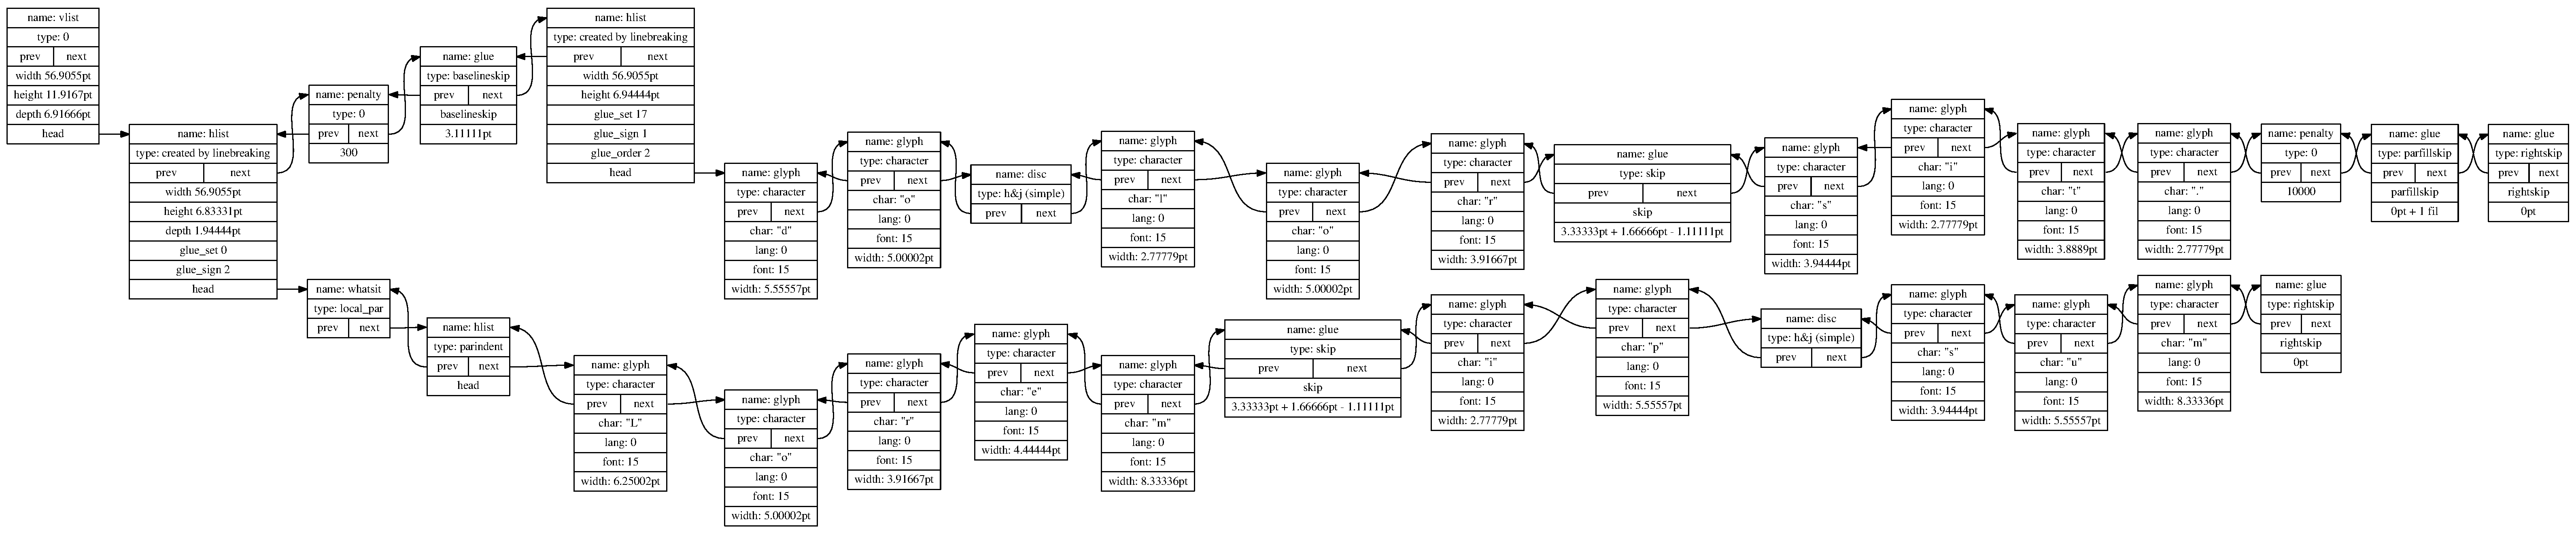
\includegraphics[width=\linewidth]{graphics/par}

\subsection{Tabular environment}

\noindent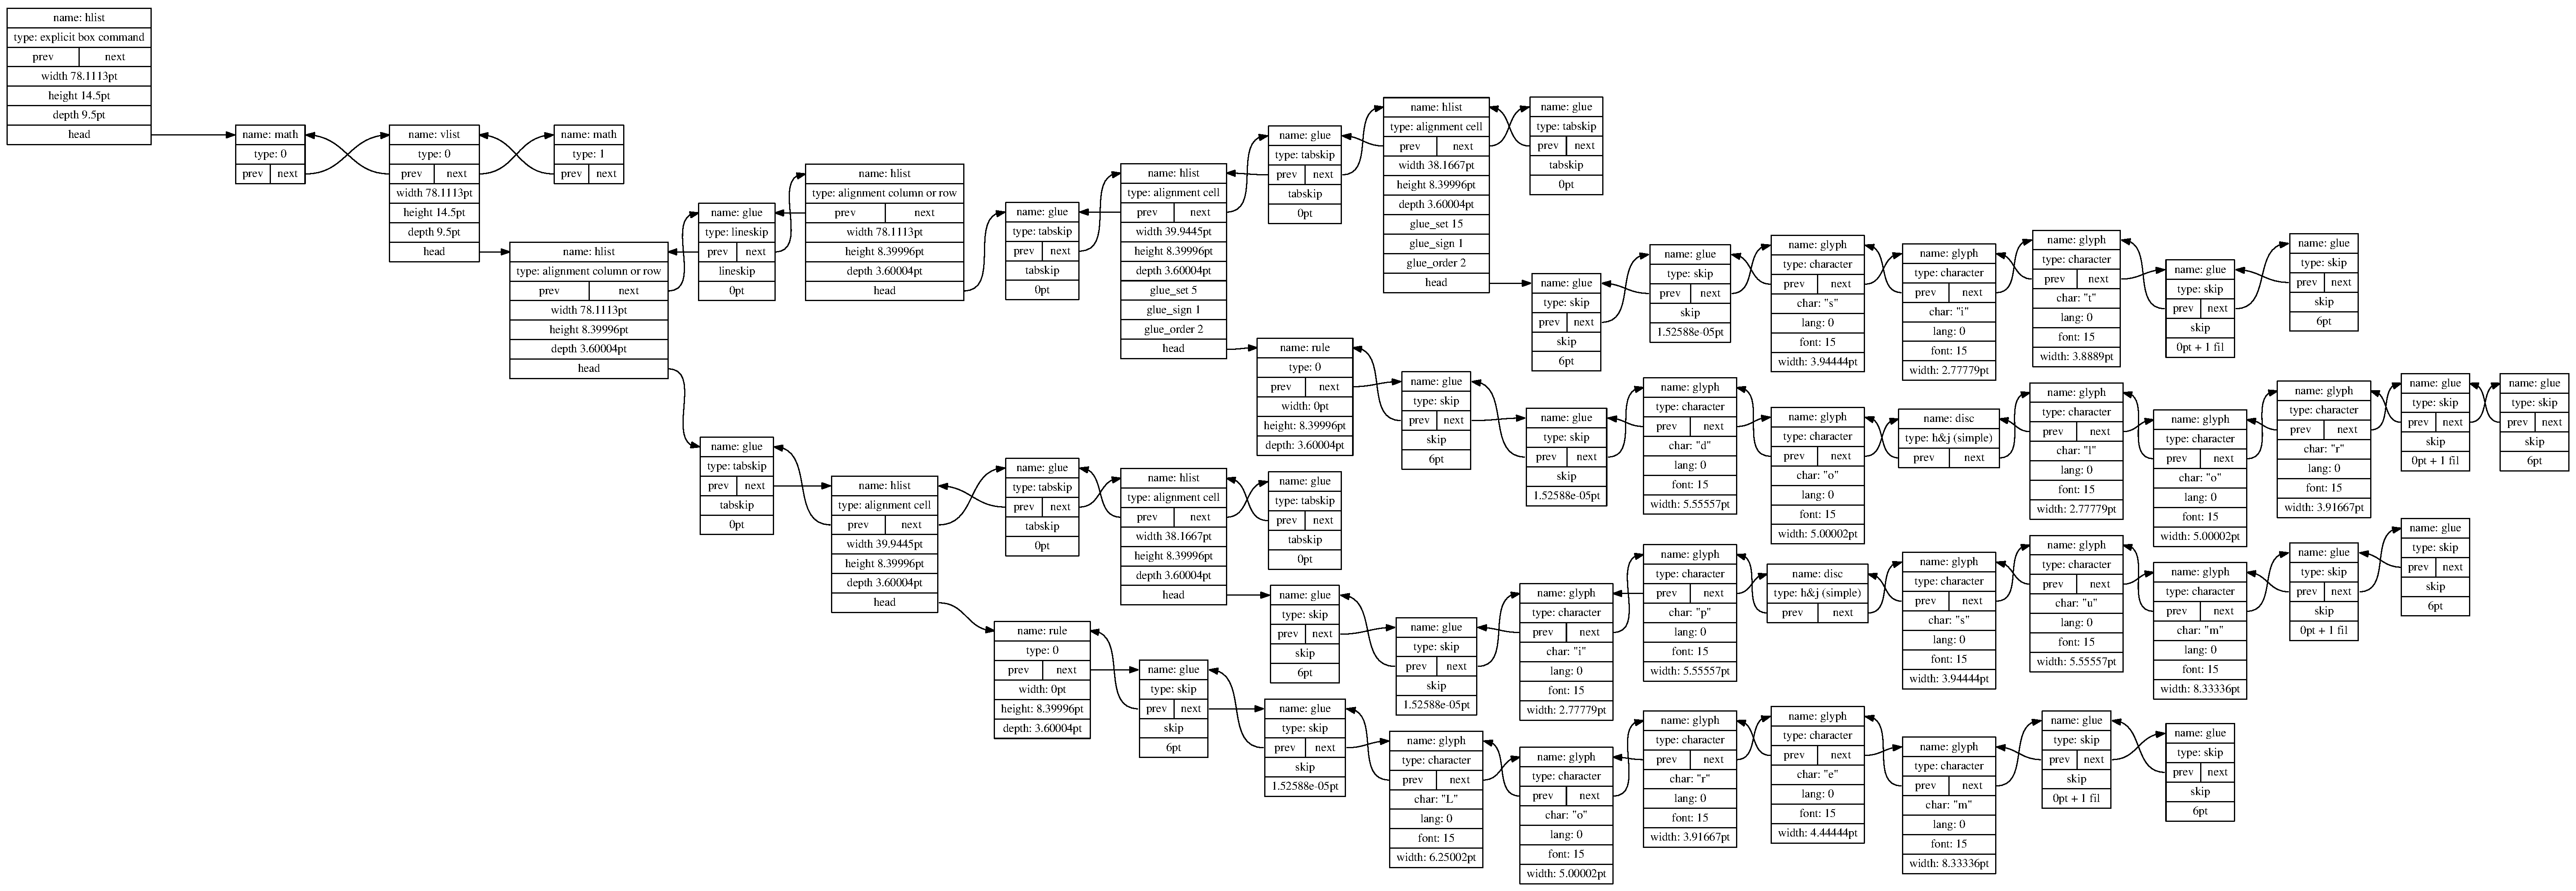
\includegraphics[width=\linewidth]{graphics/tabular}

\subsection{Picture environment}

\noindent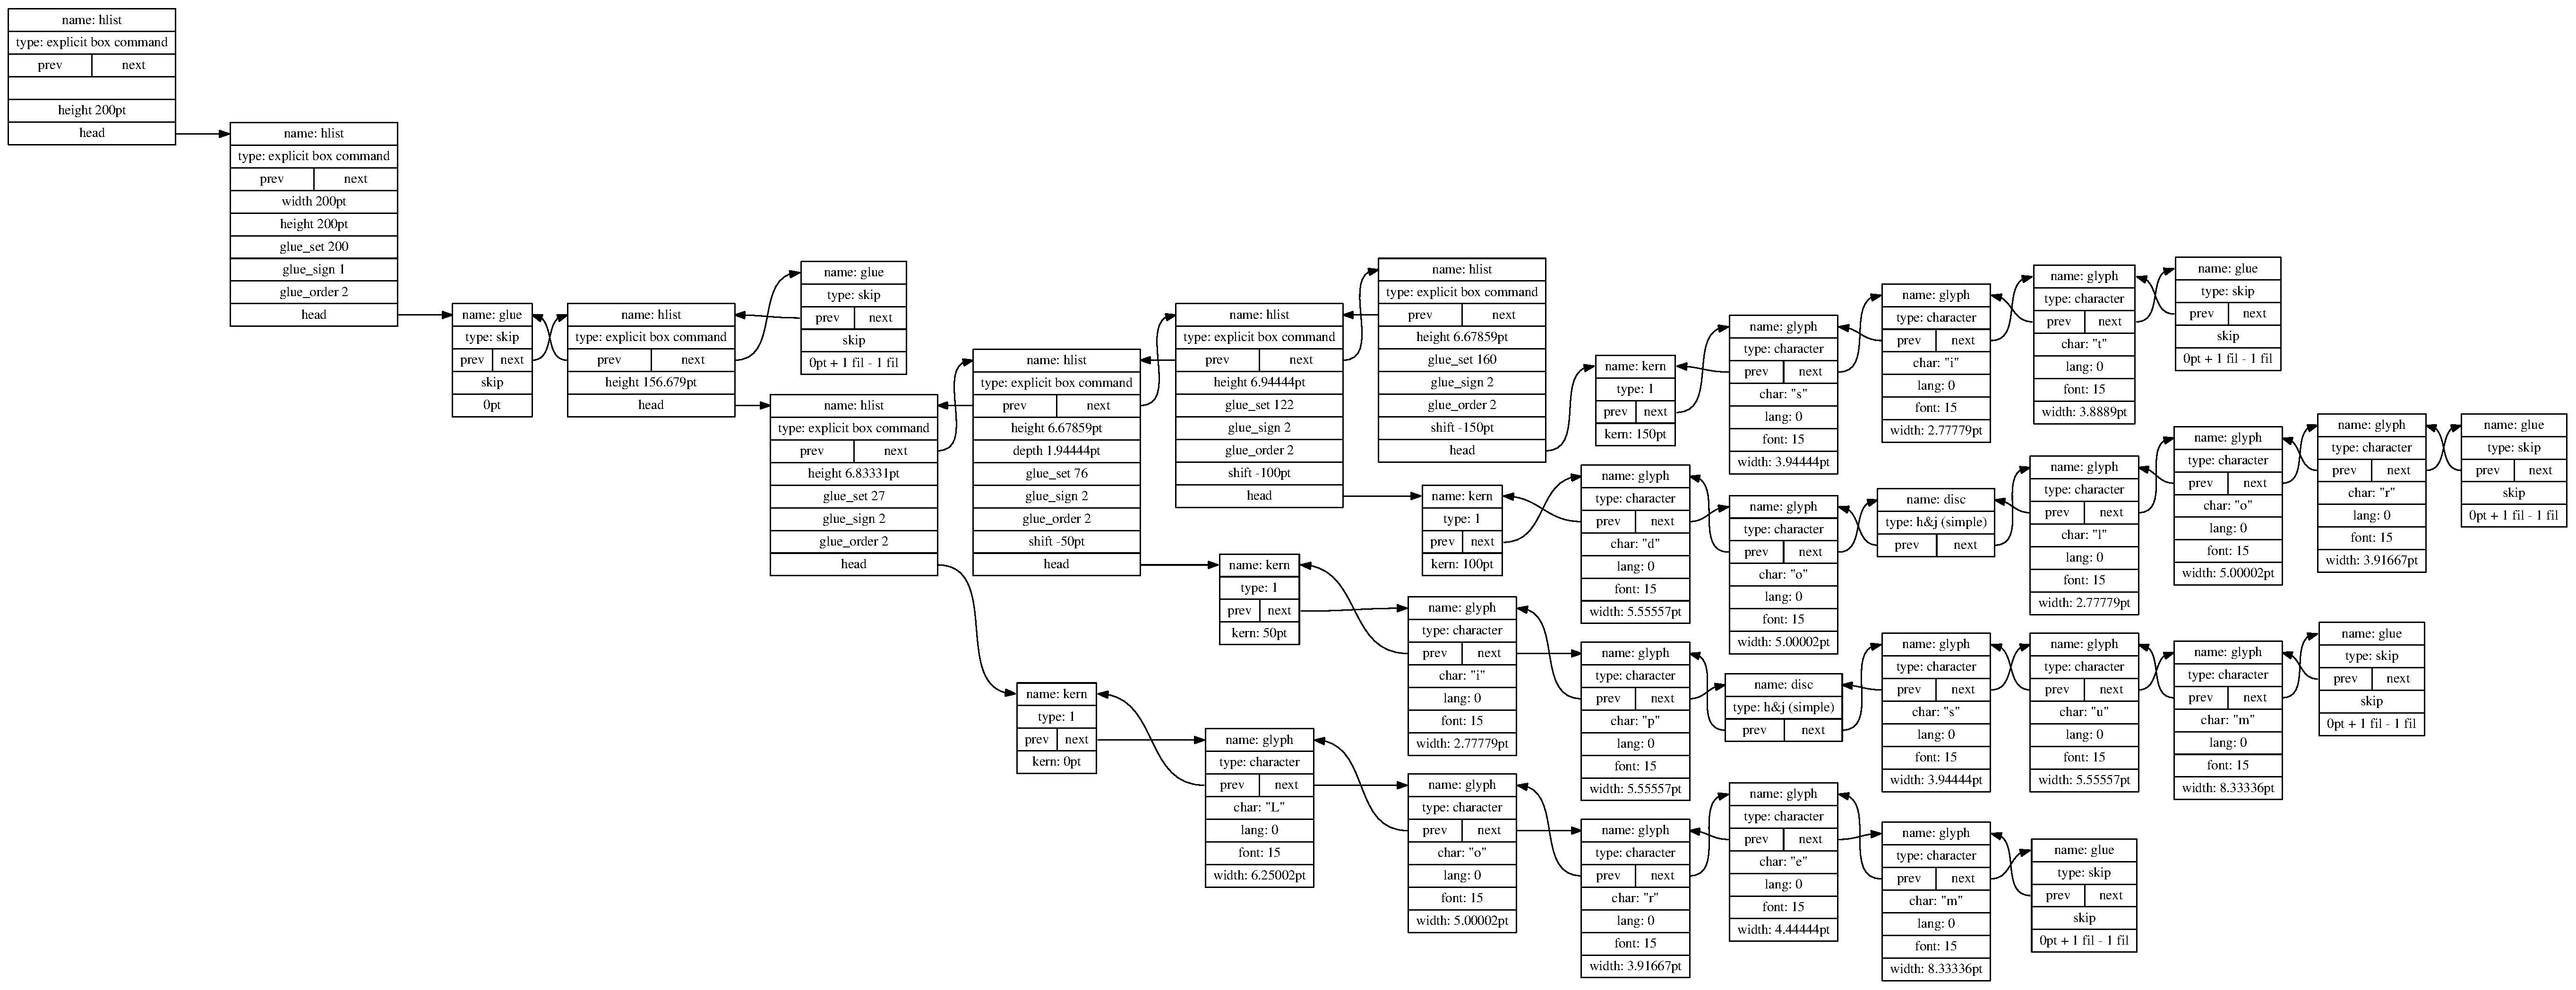
\includegraphics[width=\linewidth]{graphics/picture}

\DocInput{cloze.dtx}

\subsection{The file cloze.lua}

\inputminted{lua}{cloze.lua}

\pagebreak
\PrintChanges
\pagebreak
\PrintIndex
\end{document}
%</driver>
% \fi
%
% \CheckSum{0}
%
% \CharacterTable
%  {Upper-case    \A\B\C\D\E\F\G\H\I\J\K\L\M\N\O\P\Q\R\S\T\U\V\W\X\Y\Z
%   Lower-case    \a\b\c\d\e\f\g\h\i\j\k\l\m\n\o\p\q\r\s\t\u\v\w\x\y\z
%   Digits        \0\1\2\3\4\5\6\7\8\9
%   Exclamation   \!     Double quote  \"     Hash (number) \#
%   Dollar        \$     Percent       \%     Ampersand     \&
%   Acute accent  \'     Left paren    \(     Right paren   \)
%   Asterisk      \*     Plus          \+     Comma         \,
%   Minus         \-     Point         \.     Solidus       \/
%   Colon         \:     Semicolon     \;     Less than     \<
%   Equals        \=     Greater than  \>     Question mark \?
%   Commercial at \@     Left bracket  \[     Backslash     \\
%   Right bracket \]     Circumflex    \^     Underscore    \_
%   Grave accent  \`     Left brace    \{     Vertical bar  \|
%   Right brace   \}     Tilde         \~}
%
%
% \changes{v0.1}{2015/06/16}{Converted to DTX file}
%
% \changes{v1.0}{2015/07/08}{Inital release}
%
% \changes{v1.1}{2016/06/13}{Make cloze compatible to LuaTeX version
% 0.95}
%
% \changes{v1.2}{2016/06/23}{The cloze makros are now working in
% tabular, tabbing and picture environments}
%
% \changes{v1.3}{2017/03/13}{Add the new macros \cmd{\clozenol} and
% \cmd{\clozeextend} and the environments \texttt{clozebox} and
% \texttt{clozespace} (This version was not published on CTAN.)}
%
% \changes{v1.4}{2020/05/20}{Add the new macro \cmd{\clozestrike} and
% improve the documentation}
%
% \changes{v1.5}{2020/05/27}{
% The Lua part of the package (cloze.lua) is now being developed in a
% separate file.
% The readme file is now a standalone mardown file and not embedded in
% the dtx file any more.
% \href{https://github.com/stevedonovan/LDoc}{LDoc} is being used
% to generate
% \href{https://josef-friedrich.github.io/cloze}{source code documentation}.
% This version fixes two bugs (cloze in display math, line color and
% hide).
% }
%
% \DoNotIndex{\newcommand,\newenvironment,\def,\directlua}
%
% \StopEventually{}
% \pagebreak
% \section{Implementation}
%
% \iffalse
%<*package>
% \fi
% \MacroTopsep = 10pt plus 2pt minus 2pt
% \MacrocodeTopsep = 10pt plus 1.2pt minus 1pt
%
% \makeatletter
% \c@CodelineNo 25 \relax
% \makeatother
%
% \subsection{The file \tt{cloze.sty}}
%
% This packages are used to build \emph{cloze}:
%
% \subsubsection{Dependencies}
%
% The package \href{https://www.ctan.org/pkg/fontspec}{fontspec} is not
% necessarily required. When using Lua\LaTeX{} it is good form to load
% it. Apart from this the package supplies helpful messages, when you
% compile a Lua\LaTeX{} document with pdf\LaTeX{}.
%    \begin{macrocode}
\RequirePackage{fontspec}
%    \end{macrocode}
% The package \href{https://www.ctan.org/pkg/luatexbase}{luatexbase}
% allows to register multiple Lua callbacks.
%    \begin{macrocode}
\RequirePackage{luatexbase-mcb}
%    \end{macrocode}
% The package \href{https://www.ctan.org/pkg/kvoptions}{kvoptions}
% takes the handling of the options.
%    \begin{macrocode}
\RequirePackage{kvoptions}
%    \end{macrocode}
% The package \href{https://www.ctan.org/pkg/setspace}{setspace} is used
% by the environment |clozespace|.
%    \begin{macrocode}
\RequirePackage{setspace}
%    \end{macrocode}
% The package \href{https://www.ctan.org/pkg/xcolor}{xcolor} is required
% to colorize the text and the line of a gap.
%    \begin{macrocode}
\RequirePackage{xcolor}
%    \end{macrocode}
% The package \href{https://www.ctan.org/pkg/xcolor}{xparse} is used by
% the environment |clozebox|.
%    \begin{macrocode}
\RequirePackage{xparse}
%    \end{macrocode}
% The package \href{https://www.ctan.org/pkg/stackengine}{stackengine}
% is required by the command |\clozestrike{}{}|.
%    \begin{macrocode}
\RequirePackage{stackengine}
%    \end{macrocode}
% The package \href{https://www.ctan.org/pkg/ulem}{ulem} is required by
% the command |\clozestrike{}{}|.
%    \begin{macrocode}
\RequirePackage{ulem}
\normalem
%    \end{macrocode}
%
%    \begin{macrocode}
\RequirePackage{transparent}
%    \end{macrocode}
%
% Load the cloze lua module and put all return values in the variable
% |cloze|.
%
%    \begin{macrocode}
\directlua{
  cloze = require('cloze')
}
%    \end{macrocode}
%
%    \begin{macrocode}
\newif\ifclozeshow\clozeshowtrue
%    \end{macrocode}
%
% \subsubsection{Internal macros}
%
% \begin{macro}{\cloze@set@to@global}
% Set the Lua variable |registry.is_global| to |true|. All options
% are then stored in the variable |registry.global_options|.
%    \begin{macrocode}
\def\cloze@set@to@global{%
 \directlua{cloze.set_is_global(true)}%
}
%    \end{macrocode}
% \end{macro}
%
% \begin{macro}{\cloze@set@to@local}
% First unset the variable |registry.local_options|. Now set the Lua
% variable |registry.is_global| to |false|. All options are then stored
% in the variable |registry.local_options|.
%    \begin{macrocode}
\def\cloze@set@to@local{%
  \directlua{
    cloze.unset_local_options()
    cloze.set_is_global(false)
  }%
}
%    \end{macrocode}
% \end{macro}
%
% \begin{macro}{\cloze@set@option}
% \cmd{\cloze@set@option} is a wrapper for the Lua function
% |registry.set_option|. \cmd{\cloze@set@option}\oarg{key}\marg{value}
% sets a key \meta{key} to the value \meta{value}.
%    \begin{macrocode}
\def\cloze@set@option[#1]#2{%
  \directlua{cloze.set_option('#1', '#2')}%
}
%    \end{macrocode}
% \end{macro}
%
% \begin{macro}{\cloze@color}
% Convert a color definiton name to a PDF colorstack string, for example
% convert the color name |blue| to the colorstack string
% |0 0 1 rg 0 0 1 RG|. The macro definition |\cloze@color{blue}|
% builds itself the macro |\color@blue|, which expands to the PDF
% colorstack string. The colorstack string is necessary to generate a
% PDF colorstack whatsit.
%    \begin{macrocode}
\def\cloze@color#1{\csname\string\color@#1\endcsname}
%    \end{macrocode}
% \end{macro}
%
% \begin{macro}{\cloze@set@local@options}
% This macro is used in all cloze commands to handle the optional
% arguments. First it sets the option storage to local and then it
% commits the options to the package \emph{kvoptions} via the macro
% |\kvsetkeys{CLZ}{}|.
%    \begin{macrocode}
\def\cloze@set@local@options#1{%
  \cloze@set@to@local%
  \kvsetkeys{CLZ}{#1}%
}
%    \end{macrocode}
% \end{macro}
%
% \begin{macro}{\cloze@start@marker}
% At the begining |\cloze@start@marker| registers the required Lua
% callbacks. Then it inserts a whatsit marker which marks the begin of a
% gap.
%    \begin{macrocode}
\def\cloze@start@marker#1{%
  \strut\directlua{
    cloze.register('#1')
    cloze.marker('#1', 'start')
  }%
}
%    \end{macrocode}
% \end{macro}
%
% \begin{macro}{\cloze@stop@marker}
% \cmd{\cloze@stop@marker} inserts a whatsit marker that marks the end
% of gap.
%    \begin{macrocode}
\def\cloze@stop@marker#1{%
  \strut\directlua{
    cloze.marker('#1', 'stop')
  }%
}
%    \end{macrocode}
% \end{macro}
%
% \begin{macro}{\cloze@margin}
% \cmd{\cloze@margin} surrounds a text in a gap with two |kerns|.
%    \begin{macrocode}
\def\cloze@margin#1{%
  \directlua{cloze.margin()}%
  #1%
  \directlua{cloze.margin()}%
}
%    \end{macrocode}
% \end{macro}
%
% \subsubsection{Options}
%
% \emph{cloze} offers key-value pairs to use as options. For processing
% the key-value pairs we use the package
% \href{https://www.ctan.org/pkg/kvoptions}{kvoptions}.
% To make all key-value pairs accessibly to Lua code, we use the
% declaration
% \cmd{\define@key}\marg{CLZ}\marg{option}\oarg[]\marg{\dots}. This
% declaration comes from the package
% \href{https://www.ctan.org/pkg/keyval}{keyval}.
%
% At start all values are declared as global options. At the Lua side
% all values are now stored in the |registry.global_options| table.
%
%    \begin{macrocode}
\cloze@set@to@global
%    \end{macrocode}
%
% We use the abbreviation |CLZ| for \emph{cloze} as family name and
% prefix.
%
%    \begin{macrocode}
\SetupKeyvalOptions{
  family=CLZ,
  prefix=CLZ@
}
%    \end{macrocode}
%
% \paragraph{\tt{align}}
%
% \noindent Please read the section \secref{sec:option-align} how to use
% the option |align|. |align| affects only the command \cmd{\clozefix}
% \secref{sec:command-clozefix}.
%
%    \begin{macrocode}
\DeclareStringOption{align}
\define@key{CLZ}{align}[]{\cloze@set@option[align]{#1}}
%    \end{macrocode}
%
% \paragraph{\tt{boxheight}}
%
% \noindent Please read the section \secref{sec:sec:command-clozebox}
% how to use the option |boxheight|. |boxheight| affects only the
% environment \cmd{clozebox}.
% \secref{sec:command-clozefix}.
%
%    \begin{macrocode}
\DeclareStringOption{boxheight}
\define@key{CLZ}{boxheight}[]{\cloze@set@option[boxheight]{#1}}
%    \end{macrocode}
%
% \paragraph{\tt{boxwidth}}
%
% \noindent Please read the section \secref{sec:sec:command-clozebox}
% how to use the option |boxwidth|. |boxwidth| affects only the
% environment \cmd{clozebox}.
% \secref{sec:command-clozefix}.
%
%    \begin{macrocode}
\DeclareStringOption{boxwidth}
\define@key{CLZ}{boxwidth}[]{\cloze@set@option[boxwidth]{#1}}
%    \end{macrocode}
%
% \paragraph{\tt{distance}}
%
% \noindent Please read the section \secref{sec:option-distance} how to
% use the option |distance|.
%
%    \begin{macrocode}
\DeclareStringOption{distance}
\define@key{CLZ}{distance}[]{\cloze@set@option[distance]{#1}}
%    \end{macrocode}
%
% \paragraph{\tt{hide}}
%
% \noindent If the option |hide| appears in the commands, |hide| will be
% set to \emph{true} and |show| to \emph{false} on the Lua side. Please
% read the section \secref{sec:option-hide} how to use the option
% |hide|.
%
%    \begin{macrocode}
\DeclareVoidOption{hide}{%
  \clozeshowfalse%
  \cloze@set@option[hide]{true}%
  \cloze@set@option[show]{false}%
}
%    \end{macrocode}
%
% \paragraph{\tt{linecolor}}
%
% \noindent Please read the section \secref{sec:option-linecolor} how to
% use the option |linecolor|.
%
%    \begin{macrocode}
\DeclareStringOption{linecolor}
\define@key{CLZ}{linecolor}[]{%
  \cloze@set@option[linecolor]{\cloze@color{#1}}%
  \cloze@set@option[linecolor_name]{#1}%
}
%    \end{macrocode}
%
% \paragraph{\tt{margin}}
%
% \noindent Please read the section \secref{sec:option-margin} how to
% use the option |margin|.
%
%    \begin{macrocode}
\DeclareStringOption{margin}
\define@key{CLZ}{margin}[]{\cloze@set@option[margin]{#1}}
%    \end{macrocode}
%
% \paragraph{\tt{show}}
%
% \noindent If the option |show| appears in the commands, |show| will be
% set to \emph{true} and |true| to \emph{false} on the Lua side. Please
% read the section \secref{sec:option-show} how to use the option
% |show|.
%
%    \begin{macrocode}
\DeclareVoidOption{show}{%
  \clozeshowtrue%
  \cloze@set@option[show]{true}%
  \cloze@set@option[hide]{false}%
}
%    \end{macrocode}
%
% \paragraph{\tt{spacing}}
%
% \noindent Please read the section \secref{sec:option-spacing} how to
% use the option |spacing|.
%
%    \begin{macrocode}
\DeclareStringOption{spacing}
\define@key{CLZ}{spacing}[]{\cloze@set@option[spacing]{#1}}
%    \end{macrocode}
%
% \paragraph{\tt{textcolor}}
%
% \noindent Please read the section \secref{sec:option-textcolor} how to
% use the option |textcolor|.
%
%    \begin{macrocode}
\DeclareStringOption{textcolor}
\define@key{CLZ}{textcolor}[]{%
  \cloze@set@option[textcolor]{\cloze@color{#1}}%
  \cloze@set@option[textcolor_name]{#1}%
}
%    \end{macrocode}
%
% \paragraph{\tt{thickness}}
%
% \noindent Please read the section \secref{sec:option-thickness} how to
% use the option |thickness|.
%
%    \begin{macrocode}
\DeclareStringOption{thickness}
\define@key{CLZ}{thickness}[]{\cloze@set@option[thickness]{#1}}
%    \end{macrocode}
%
% \paragraph{\tt{width}}
%
% \noindent Please read the section \secref{sec:option-width} how to use
% the option |width|. |width| affects only the command \cmd{\clozefix}
% \secref{sec:command-clozefix}.
%
%    \begin{macrocode}
\DeclareStringOption{width}
\define@key{CLZ}{width}[]{\cloze@set@option[width]{#1}}
%    \end{macrocode}
%
%    \begin{macrocode}
\ProcessKeyvalOptions{CLZ}
%    \end{macrocode}
%
% \subsubsection{Public macros}
%
% All public macros are prefixed with |\cloze|.
%
% \begin{macro}{\clozeset}
% The usage of the command \cmd{\clozeset} is described in detail in
% section \secref{sec:command-clozeset}.
%    \begin{macrocode}
\newcommand{\clozeset}[1]{%
  \cloze@set@to@global%
  \kvsetkeys{CLZ}{#1}%
}
%    \end{macrocode}
% \end{macro}
%
% \begin{macro}{\clozereset}
% The usage of the command \cmd{\clozereset} is described in detail in
% section \secref{sec:command-clozereset}.
%    \begin{macrocode}
\newcommand{\clozereset}{%
  \directlua{cloze.reset()}
}
%    \end{macrocode}
% \end{macro}
%
% \begin{macro}{\clozeshow}
% The usage of the command \cmd{\clozeshow} is described in detail in
% section \secref{sec:command-clozeshow}.
%    \begin{macrocode}
\newcommand{\clozeshow}{%
  \clozeset{show}
}
%    \end{macrocode}
% \end{macro}
%
% \begin{macro}{\clozehide}
% The usage of the command \cmd{\clozehide} is described in detail in
% section \secref{sec:command-clozehide}.
%    \begin{macrocode}
\newcommand{\clozehide}{%
  \clozeset{hide}
}
%    \end{macrocode}
% \end{macro}
%
% \begin{macro}{\clozefont}
% The usage of the command \cmd{\clozefont} is described in detail in
% section \secref{sec:command-clozefont}.
%    \begin{macrocode}
\newcommand{\clozefont}{\itshape}
%    \end{macrocode}
% \end{macro}
%
% \begin{macro}{\clozesetfont}
% The usage of the command \cmd{\clozesetfont} is described in detail in
% section \secref{sec:command-clozesetfont}.
%    \begin{macrocode}
\newcommand{\clozesetfont}[1]{%
  \renewcommand{\clozefont}[1]{%
    #1%
  }%
}
%    \end{macrocode}
% \end{macro}
%
% \begin{macro}{\cloze}
% The usage of the command \cmd{\cloze} is described in detail in
% section \secref{sec:command-cloze}.
%    \begin{macrocode}
\newcommand{\cloze}[2][]{%
  \cloze@set@local@options{#1}%
  \cloze@start@marker{basic}%
  {%
    \clozefont\relax%
    \cloze@margin{#2}%
  }%
  \cloze@stop@marker{basic}%
}
%    \end{macrocode}
% \end{macro}
%
% \begin{macro}{\clozefix}
% The usage of the command \cmd{\clozefix} is described in detail in
% section \secref{sec:command-clozefix}.
%    \begin{macrocode}
\newcommand{\clozefix}[2][]{%
  \cloze@set@local@options{#1}%
  \cloze@start@marker{fix}%
  {%
    \clozefont\relax%
    \cloze@margin{#2}%
  }%
  \cloze@stop@marker{fix}%
}
%    \end{macrocode}
% \end{macro}
%
% \begin{macro}{\clozenol}
% The usage of the command \cmd{\clozenol} is described in detail in
% section \secref{sec:command-clozenol}.
% TODO: Realize this macro with lua code, without ugly |\color{white}|.
% command.
%    \begin{macrocode}
\newcommand{\clozenol}[2][]{%
  {%
    \cloze@set@local@options{#1}%
    \clozefont\relax%
    \ifclozeshow%
      \color{\directlua{tex.print(cloze.get_value('textcolor_name'))}}%
    \else%
      \color{white}%
    \fi%
    #2%
  }%
}
%    \end{macrocode}
% \end{macro}
%
% \begin{environment}{clozepar}
% The usage of the environment |clozepar| is described in detail in
% section \secref{sec:command-clozepar}.
%    \begin{macrocode}
\newenvironment{clozepar}[1][]%
{%
  \par%
  \cloze@set@local@options{#1}%
  \cloze@start@marker{par}%
  \clozefont\relax%
}%
{%
  \cloze@stop@marker{par}%
  \par%
  \directlua{cloze.unregister('par')}%
}
%    \end{macrocode}
% \end{environment}
%
% \begin{macro}{\cloze@get@value}
%    \begin{macrocode}
\newcommand{\cloze@get@value}[1]{%
  \directlua{
    tex.print(cloze.get_value('#1'))
  }%
}
%    \end{macrocode}
% \end{macro}
%
% \begin{environment}{clozebox}
% The usage of the environment |clozebox| is described in detail in
% section \secref{sec:command-clozebox}.
% TODO: Realize this macro with lua code, without ugly |\color{white}|
% command.
%    \begin{macrocode}
\newsavebox{\cloze@box}
\NewDocumentEnvironment{clozebox}{ s O{} +b}{%
  \cloze@set@local@options{#2}%
  \noindent%
  \begin{lrbox}{\cloze@box}%
  \directlua{
    local boxheight = cloze.get_value('boxheight')
    local boxwidth = cloze.get_value('boxwidth')
    if boxheight then
      tex.print('\\begin{minipage}[t][' .. boxheight .. '][t]{' .. boxwidth .. '}')
    else
      tex.print('\\begin{minipage}[t]{' .. boxwidth .. '}')
    end
  }
    \clozefont\relax%
    \ifclozeshow%
      \color{\directlua{tex.print(cloze.get_value('textcolor_name'))}}#3%
    \else%
      \color{white}#3%
    \fi%
  \end{minipage}%
  \end{lrbox}%
  \IfBooleanTF{#1}%
    {\usebox{\cloze@box}}%
    {\fbox{\usebox{\cloze@box}}}%
}{}
%    \end{macrocode}
% \end{environment}
%
% \begin{environment}{clozespace}
% The usage of the environment |clozespace| is described in detail in
% section \secref{sec:command-clozespace}.
% TODO: Realization without setspace package.
%    \begin{macrocode}
\newenvironment{clozespace}[1][]%
{%
  \cloze@set@local@options{#1}%
  \begin{spacing}{\directlua{tex.print(cloze.get_value('spacing'))}}%
}{\end{spacing}}
%    \end{macrocode}
% \end{environment}
%
% \begin{macro}{\clozefil}
% The usage of the command \cmd{\clozefil} is described in detail in
% section \secref{sec:command-clozefil}.
%    \begin{macrocode}
\newcommand{\clozefil}[2][]{%
  \cloze[#1]{#2}\clozelinefil[#1]%
}
%    \end{macrocode}
% \end{macro}
%
% \begin{macro}{\clozeextend}
% TODO: Use node library to create kern nodes.
%    \begin{macrocode}
\newcommand{\clozeextend}[1][1]{%
  \directlua{
    local loop = #1
    for variable = 1, loop do
      tex.print(' \string\\hspace{1em} \string\\strut')
    end
  }
}
%    \end{macrocode}
% \end{macro}
%
% \begin{macro}{\clozeline}
% The usage of the command \cmd{\clozeline} is described in detail in
% section \secref{sec:command-clozeline}.
%    \begin{macrocode}
\newcommand{\clozeline}[1][]{%
  \cloze@set@local@options{#1}%
  \directlua{cloze.line()}%
}
%    \end{macrocode}
% \end{macro}
%
% \begin{macro}{\clozelinefil}
% The usage of the command \cmd{\clozelinefil} is described in detail in
% section \secref{sec:command-clozelinefil}.
%    \begin{macrocode}
\newcommand{\clozelinefil}[1][]{%
  \cloze@set@local@options{#1}%
  \strut%
  \directlua{cloze.linefil()}%
  \strut%
}
%    \end{macrocode}
% \end{macro}
%
% \begin{macro}{\cloze@text@color}
%    \begin{macrocode}
\newcommand{\cloze@text@color}[1]{%
  \textcolor%
    {\directlua{tex.print(cloze.get_value('textcolor_name'))}}%
    {#1}%
}
%    \end{macrocode}
% \end{macro}
%
% \begin{macro}{\cloze@strike@line}
%    \begin{macrocode}
\newcommand\cloze@strike@line{%
  \bgroup%
  \markoverwith{%
    \cloze@text@color{%
      \rule[0.5ex]{2pt}{1pt}%
    }%
  }%
  \ULon%
}
%    \end{macrocode}
% \end{macro}
%
% \begin{macro}{\clozestrike}
%    \begin{macrocode}
\newcommand{\clozestrike}[3][]{%
  \cloze@set@local@options{#1}%
  \ifclozeshow%
    \stackengine%
      {\Sstackgap}% \Sstackgap or \Lstackgap or \stackgap or stacklength
      {\cloze@strike@line{#2}}% anchor
      {\cloze@text@color{\clozefont{}#3}}% item
      {O}% O or U
      {c}% \stackalignment or l or c or r
      {\quietstack}% \quietstack or T or F
      {T}% \useanchorwidth or T or F
      {\stacktype}% \stacktype or S or L
  \else%
    \stackengine%
      {\Sstackgap}% \Sstackgap or \Lstackgap or \stackgap or stacklength
      {#2}% anchor
      {\texttransparent{0}{\clozefont{}#3}}% item
      {O}% O or U
      {c}% \stackalignment or l or c or r
      {\quietstack}% \quietstack or T or F
      {T}% \useanchorwidth or T or F
      {\stacktype}% \stacktype or S or L
  \fi%
}
%    \end{macrocode}
% \end{macro}
%
% \iffalse
%</package>
% \fi
%
% \Finale
\endinput
